\begin{center}

\includegraphics[width=0.6\textwidth]{content/3/chapter4/images/36.png}\\
Cippi admires the diamond
\end{center}

With C++20, we get two new keywords: consteval and constinit. Keyword consteval produces a function that is executed at compile time and constinit guarantees that a variable is initialized at compile time. Now, you may have the impression that both specifiers are quite similar to constexpr. To make it short, you are right. Before I compare the keywords consteval, constinit, constexpr, and good old const, I have to introduce the new specifiers consteval and constinit.


\subsubsubsection{4.5.1\hspace{0.2cm} consteval}

consteval creates a so-called immediate function.

\hspace*{\fill} \\ %插入空行
\noindent
A consteval function
\begin{lstlisting}[style=styleCXX]
consteval int sqr(int n) {
	return n * n;
}
\end{lstlisting}

Each invocation of an immediate function creates a compile-time constant. To say it more directly, a consteval (immediate) function is executed at compile time.

consteval cannot be applied to destructors or functions that allocate or deallocate. You can only use at most one of consteval, constexpr, or constinit specifier in a declaration. An immediate function (consteval) is implicitly inline and has to fulfill the requirements for a constexpr function.

The requirements of a constexpr function in C++14 and, therefore, a consteval function:

\begin{itemize}
\item 
A consteval (constexpr) can
\begin{itemize}
\item 
have conditional jump instructions or loop instructions.

\item 
have more than one instruction.

\item 
invoke constexpr functions. A consteval function can only invoke a constexpr function but not the other way around.

\item 
use fundamental data types as variables that have to be initialized with a constant expression.
\end{itemize}

\item 
A consteval (constexpr) function cannot
\begin{itemize}
\item 
have static or thread\_local data.

\item 
have a try block nor a goto instruction.

\item 
invoke or use non-consteval functions or non-constexpr data.
\end{itemize}
\end{itemize}

To make it short: all dependencies of a consteval function must be resolved at compile time.

The program constevalSqr.cpp applies the consteval function sqr.

\hspace*{\fill} \\ %插入空行
\noindent
A consteval function
\begin{lstlisting}[style=styleCXX]
// constevalSqr.cpp

#include <iostream>

consteval int sqr(int n) {
	return n * n;
}

int main() {

	std::cout << "sqr(5): " << sqr(5) << '\n';
	
	const int a = 5;
	std::cout << "sqr(a): " << sqr(a) << '\n';
	
	int b = 5;
	// std::cout << "sqr(b): " << sqr(b) << '\n'; ERROR

}
\end{lstlisting}

The number 5 is a constant expression and can be used as an argument for the function sqr (line 11). The same holds for the variable a (line 13). A constant variable such as a is usable in a constant expression when it is initialized with a constant expression. The variable b (line 16) is not a constant expression. Consequently, the invocation of sqr(b) (line 17) is not valid.

Here is the output of the program:

\begin{tcblisting}{commandshell={}}
sqr(5): 25
sqr(a): 25
\end{tcblisting}

\begin{center}
Use of a consteval function
\end{center}

\subsubsubsection{4.5.2\hspace{0.2cm} constinit}

constinit can be applied to variables with static storage duration or thread storage duration.

\begin{itemize}
\item 
Global (namespace) variables, static variables, or static class members have static storage duration. These objects are allocated when the program starts, and are deallocated when the program ends.

\item 
thread\_local variables have thread storage duration. Thread-local data is created for each thread that uses this data. thread\_local data exclusively belongs to the thread. They are created at its first usage and its lifetime is bound to the lifetime of the thread it belongs to. Often threadlocal data is called thread-local storage.
\end{itemize}

constinit ensures for this kind of variable (static storage duration or thread storage duration) that it is initialized at compile time. constinit does not imply constness.

\hspace*{\fill} \\ %插入空行
\noindent
Initialization with constinit
\begin{lstlisting}[style=styleCXX]
// constinitSqr.cpp
#include <iostream>
consteval int sqr(int n) {
	return n * n;
}
constexpr auto res1 = sqr(5);
constinit auto res2 = sqr(5);
int main() {
	std::cout << "sqr(5): " << res1 << '\n';
	std::cout << "sqr(5): " << res2 << '\n';
	constinit thread_local auto res3 = sqr(5);
	std::cout << "sqr(5): " << res3 << '\n';
}
\end{lstlisting}

res1 and res2 have static storage duration. res3 has thread storage duration.

\begin{tcblisting}{commandshell={}}
sqr(5): 25
sqr(5): 25
sqr(5): 25
\end{tcblisting}

\begin{center}
Use of constinit initialization
\end{center}

Now it’s time to write about the differences between const, constexpr, consteval, and constinit.

First, I discuss function execution and then variable initialization.

\subsubsubsection{4.5.3\hspace{0.2cm} Function Execution}

The following program consteval.cpp has three versions of a square function.

\hspace*{\fill} \\ %插入空行
\noindent
Three versions of a square function
\begin{lstlisting}[style=styleCXX]
// consteval.cpp

#include <iostream>

int sqrRunTime(int n) {
	return n * n;
}

consteval int sqrCompileTime(int n) {
	return n * n;
}

constexpr int sqrRunOrCompileTime(int n) {
	return n * n;
}

int main() {

	// constexpr int prod1 = sqrRunTime(100); ERROR
	constexpr int prod2 = sqrCompileTime(100);
	constexpr int prod3 = sqrRunOrCompileTime(100);

	int x = 100;
	
	int prod4 = sqrRunTime(x);
	// int prod5 = sqrCompileTime(x); ERROR
	int prod6 = sqrRunOrCompileTime(x);
}
\end{lstlisting}

As the name suggests: the ordinary function sqrRunTime (line 5) runs at run time, the consteval function sqrCompileTime runs at compile time (line 9), the constexpr function sqrRunOrCompileTime can run at compile time or run time. Consequently, asking for the result at compile time with sqrRunTime (line 19) is an error, accordingly, using a non-constant expression as an argument for sqrCompileTime (line 26) is also an error.

The difference between the constexpr function sqrRunOrCompileTime and the consteval function sqrCompileTime is that sqrRunOrCompileTime must be executed at compile time when the context requires compile-time evaluation.

\noindent
Compile-time and run-time execution
\begin{lstlisting}[style=styleCXX]
static_assert(sqrRunOrCompileTime(10) == 100); // compile time
int arrayNewWithConstExpressiomFunction[sqrRunOrCompileTime(100)]; // compile time
constexpr int prod = sqrRunOrCompileTime(100); // compile time

int a = 100;
int runTime = sqrRunOrCompileTime(a); // run time

int runTimeOrCompiletime = sqrRunOrCompileTime(100); // run time or compile time

int alwaysCompileTime = sqrCompileTime(100); // compile time
\end{lstlisting}

The lines 1 - 3 require compile-time evaluation. Line 6 can only be evaluated at run time because a is not a constant expression. The critical line is line 8. The function can be executed at compile time or run time. Whether it is executed at compile time or run time may depend on the compiler or on the optimization level. This observation does not hold for line 10. A consteval function is always executed at compile time.

\subsubsubsection{4.5.4\hspace{0.2cm} Variable Initialization}

The program constexprConstinit.cpp compares const, constexpr, and constinit.

\hspace*{\fill} \\ %插入空行
\noindent
Comparison of const, constexpr, and constinit
\begin{lstlisting}[style=styleCXX]
// constexprConstinit.cpp

#include <iostream>

constexpr int constexprVal = 1000;
constinit int constinitVal = 1000;

int incrementMe(int val){ return ++val;}

int main() {
	
	auto val = 1000;
	const auto res = incrementMe(val);
	std::cout << "res: " << res << '\n';
	
	// std::cout << "res: " << ++res << '\n'; ERROR
	// std::cout << "++constexprVal: " << ++constexprVal << '\n'; ERROR
	std::cout << "++constinitVal: " << ++constinitVal << '\n';
	
	constexpr auto localConstexpr = 1000;
	// constinit auto localConstinit = 1000; ERROR

}
\end{lstlisting}

Only the const variable (line 13) is initialized at run time. The constexpr and constinit variables are initialized at compile time.

The constinit (line 18) does not imply constness, as do const (line 16), or constexpr (line 17). A constexpr (line 20) or const (line 13) declared variable can be created as a local, but not a constinit declared variable (line 21).

\begin{tcblisting}{commandshell={}}
res: 1001
++constinitVal: 1001
\end{tcblisting}

\begin{center}
const, constexpr, and constinit declared variables
\end{center}

\subsubsubsection{4.5.5\hspace{0.2cm} Solving the Static Initialization Order Fiasco}

According to the \href{https://isocpp.org/wiki/faq/ctors#static-init-order}{FAQ at isocpp.org}, the static initialization order fiasco is “a subtle way to crash your program”. The FAQ continues: “The static initialization order problem is a very subtle and commonly misunderstood aspect of C++.”

Before I continue, I want to make a short disclaimer. Dependencies on variables with static storage duration (short statics) in different translation units are, in general, a code smell and should be a reason for refactoring. Consequently, if you follow my advice to refactor, you can skip this section.

\hspace*{\fill} \\ %插入空行
\noindent
4.5.5.1\hspace{0.2cm} Static Initialization Order Fiasco

Static variables in one translation unit are initialized according to their definition order.

In contrast, the initialization of static variables between translation units has a severe issue. When one static variable staticA is defined in one translation unit and another static variable staticB is defined in another translation unit, and staticB needs staticA to initialize itself, you end up with the static initialization order fiasco. The program is ill-formed because you have no guarantee which static variable is initialized first at (dynamic) run time.

Before I write about the solution, let me show you the static initialization order fiasco in action.

\hspace*{\fill} \\ %插入空行
\noindent
4.5.5.1.1\hspace{0.2cm} A 50:50 Chance to get it Right

What is unique about the initialization of statics? The initialization-order of statics happens in two steps: static and dynamic.

When a static cannot be const-initialized during compile time, it is zero-initialized. At run time, the dynamic initialization happens for these statics that were zero-initialized.

\hspace*{\fill} \\ %插入空行
\noindent
The static initialization order fiasco
\begin{lstlisting}[style=styleCXX]
// sourceSIOF1.cpp
int square(int n) {
	return n * n;
}
auto staticA = square(5);
\end{lstlisting}

\hspace*{\fill} \\ %插入空行
\noindent
The static initialization order fiasco
\begin{lstlisting}[style=styleCXX]
// mainSOIF1.cpp

#include <iostream>

extern int staticA;
auto staticB = staticA;

int main() {
	
	std::cout << '\n';
	
	std::cout << "staticB: " << staticB << '\n';
	
	std::cout << '\n';

}
\end{lstlisting}

Line 5 declares the static variable staticA. The initialization of staticB depends on the initialization of staticA. But staticB is zero-initialized at compile time and dynamically initialized at run time. The issue is that there is no guarantee in which order staticA or staticB are initialized because staticA and staticB belong to different translation units. You have a 50:50 chance that staticB is 0 or 25.

To demonstrate this problem, I can change the link order of the object files. This also changes the value for staticB!

\begin{center}
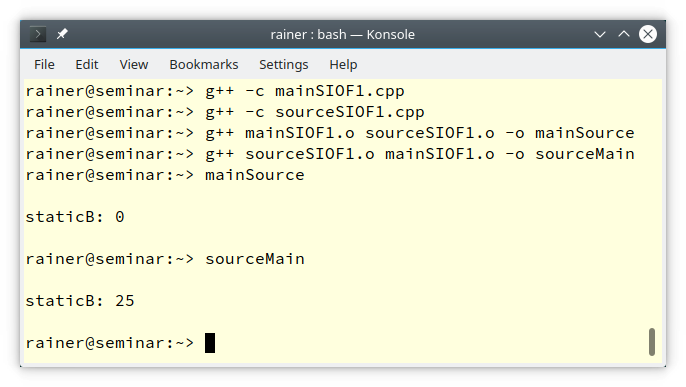
\includegraphics[width=0.6\textwidth]{content/3/chapter4/images/37.png}\\
The static initializaion order fiasco caught in action
\end{center}

What a fiasco! The result of the executable depends on the link order of the object files. What can we do when we don’t have C++20 at our disposal?

\hspace*{\fill} \\ %插入空行
\noindent
4.5.5.1.2\hspace{0.2cm} Lazy initialization of a static with a Local Scope

Static variables with local scope are created when they are used the first time. Local scope essentially means that the static variable is surrounded in some way by curly braces. This lazy creation is a guarantee that C++98 provides. With C++11, static variables with local scope are also initialized in a thread-safe way. The thread-safe \href{https://en.wikipedia.org/wiki/Scott_Meyers}{Meyers} singleton is based on this additional guarantee.

The lazy initialization can also be used to overcome the static initialization order fiasco.

\hspace*{\fill} \\ %插入空行
\noindent
Lazy initialization of a static with local scope
\begin{lstlisting}[style=styleCXX]
// sourceSIOF2.cpp

int square(int n) {
	return n * n;
}

int& staticA() {
	
	static auto staticA = square(5);
	return staticA;

}
\end{lstlisting}

\hspace*{\fill} \\ %插入空行
\noindent
Lazy initialization of a static with local scope
\begin{lstlisting}[style=styleCXX]
// mainSOIF2.cpp

#include <iostream>

int& staticA();

auto staticB = staticA();

int main() {
	
	std::cout << '\n';
	
	std::cout << "staticB: " << staticB << '\n';
	
	std::cout << '\n';

}
\end{lstlisting}

staticA (line 9 in file sourceSIOF2.cpp) is, in this case, a static in a local scope. The line 5 in file mainSOIF2.cpp declares the function staticA, which is used to initialize in the following line staticB. This local scope of staticA guarantees that staticA is created and initialized during run time when it is the first time used. Changing the link order can, in this case, not change the value of staticB.

\begin{center}
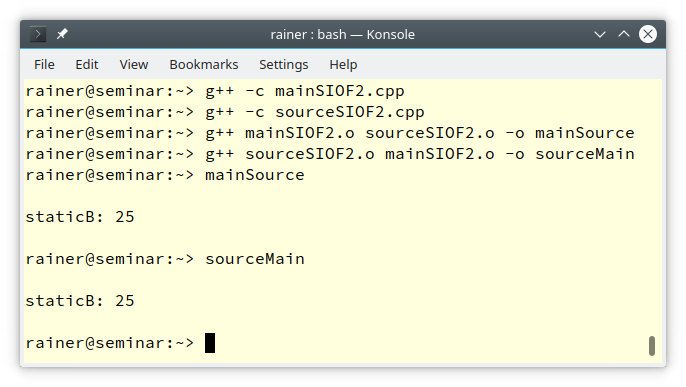
\includegraphics[width=0.6\textwidth]{content/3/chapter4/images/38.png}\\
Solving the static initialization order fiasco with local statics
\end{center}

In the last step, I solve the static initialization order fiasco using C++20.

\hspace*{\fill} \\ %插入空行
\noindent
4.5.5.1.3\hspace{0.2cm} Compile-Time Initialization of a static

Let me apply constinit to staticA. The constinit guarantees that staticA is initialized during compile time.

\hspace*{\fill} \\ %插入空行
\noindent
Compile-time initialization of a static
\begin{lstlisting}[style=styleCXX]
// sourceSIOF3.cpp

constexpr int square(int n) {
	return n * n;
}

constinit auto staticA = square(5);
\end{lstlisting}

\hspace*{\fill} \\ %插入空行
\noindent
Compile-time initialization of a static
\begin{lstlisting}[style=styleCXX]
// mainSOIF3.cpp

#include <iostream>

extern constinit int staticA;

auto staticB = staticA;

int main() {
	
	std::cout << '\n';
	
	std::cout << "staticB: " << staticB << '\n';
	
	std::cout << '\n';

}
\end{lstlisting}

Line 5 in file mainSOIF3.cpp declares the variable staticA, which is initialized (line 7 in file sourceSIOF3.cpp) at compile time. By the way, using constexpr (line 5 in file mainSOIF3.cpp) instead of constinit would not be valid, because constexpr requires a definition and not just a declaration.

\begin{center}
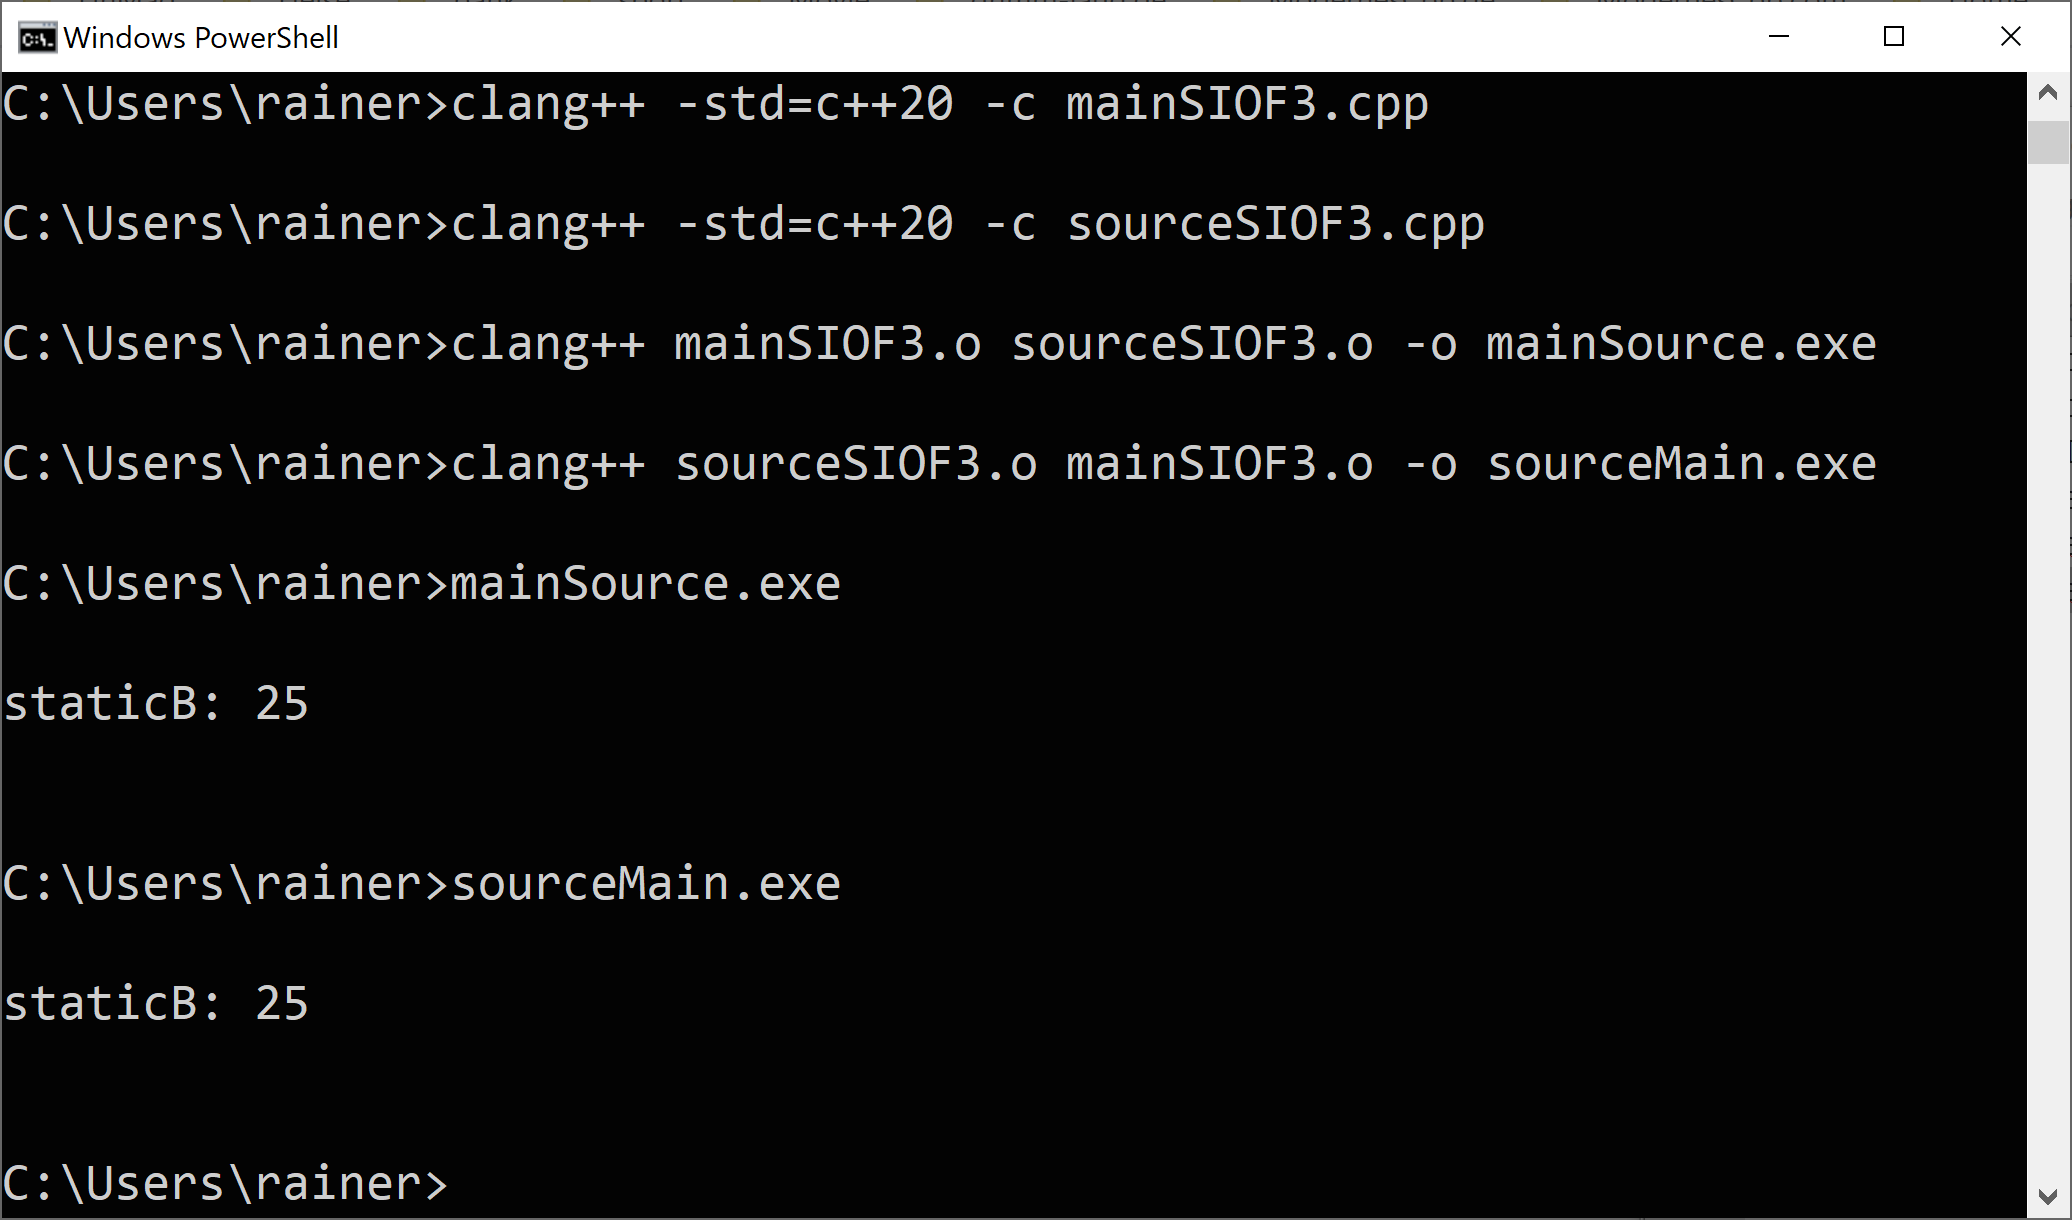
\includegraphics[width=0.6\textwidth]{content/3/chapter4/images/39.png}\\
Solving the static initializaion order fiasco with constinit
\end{center}

As in the case of the lazy initialization with a local static, staticB has the value 25.

\begin{tcolorbox}[colback=blue!5!white,colframe=blue!75!black,title={Distilled Information}]
\begin{itemize}
\item 
With C++20, we get two new keywords: consteval and constinit. consteval produces a function that is executed at compile time, and constinit guarantees that the variable is initialized at compile time.

\item 
In contrast to constexpr in C++11, consteval guarantees that the function is executed at compile time.

\item 
There are subtle differences between const, constexpr, and constinit. const and constexpr create constant variables. constexpr and constinit are executed at compile time.
\end{itemize}
\end{tcolorbox}	





